\documentclass[10pt,showpacs,preprintnumbers,footinbib,amsmath,amssymb,aps,prl,twocolumn,groupedaddress,superscriptaddress,showkeys]{revtex4-1}
\usepackage{graphicx}
\usepackage{float}
\usepackage{dcolumn}
\usepackage{bm}
\usepackage[colorlinks=true,urlcolor=blue,citecolor=blue]{hyperref}
\usepackage{color}
\usepackage{listings}

\newcommand{\deriv}[3][]{% \deriv[<order>]{<func>}{<var>}
	\ensuremath{ \frac{d^{#1} {#2}}{d {#3}^{#1}} } }


\begin{document}
\title{Building and effective field theory for neutron-proton scattering}
\author{Thomas Redpath and Dayah Chrisman}
\affiliation{Department of Physics and Astronomy, Michigan State University}
\begin{abstract}

We build an effective field theory (EFT) to describe neutron-proton scattering. We take the
underlying theory to be a sum of three Yukawa potentials with empirically derived parameters
(the potential model from the previous project). By fitting to the low energy phase shifts
($\delta _0$) calculated from solving the Lippman-Schwinger equation, we determine the
coefficients for the contact interactions in the EFT potential. We report reasonable
agreement (errors $< 10 \%$) with our underlying theory up to lab energies around 10
MeV. We find the breakdown scale
for our pionless EFT to be of order $m_{\pi}$ and roughly 3 fm$^{-1}$ for our one pion
EFT.


\end{abstract}
\maketitle

\section{Introduction}

Measuring the final states of two nucleons after they interact provides information about
the nature of their interaction. One way to summarize the information we get from these
scattering experiments is through the phase shift - which can be roughly described as a
shift in the scattered wavefunction relative to the incoming one. In this project, we create
an effective field theory to describe the nucleon scattering processes.

Effective field theories attempt to describe the low energy physics of some interaction
without exactly treating the high energy processes that act over short distances.
We describe here a simple Effective Field Theory (EFT) for neutron-proton scattering
that does not incorporate spin or isospin degrees of freedom. One key component of
an EFT is the cutoff beyond which high momentum states that are sensitive to the
unknown short-range dynamics are excluded \citep{Lepage}.
In the first version of our EFT, we treat only the physics described by the effective range
expansion. As such, we only expect our model to accurately calculate the phase shifts for
lab energies up to about 10 MeV. In the second version, we incorporate information about
the long range nuclear potential into our model in an effort to improve agreement at higher
energies with our underlying theory.


We organize this report as follows: first we summarize the forms for the EFT potentials we
use to numerically calculate the phase shifts. We then describe the framework we used to
carry out our calculations. Next, we present the results of our calcuations, and finally, we
summarize our findings and offer some comments on the work.



\section{Theory and algorithms}\label{sec:theory}

\subsection{Pionless EFT}

To begin building our pionless effective field theory, we take our underlying theory, to be
the three-Yukawa $np$ model

\begin{equation}
	V _{np}(r)=V_a \frac{e^{-ax}}{x}+V_b \frac{e^{-bx}}{x}+V_c \frac{e^{-cx}}{x},
	\label{eq:NPpot}
\end{equation}
with $x=\mu r$, $\mu=0.7$ fm$^{-1}$,
$V_a=-10.463$ MeV and $a=1$, $V_b=-1650.6$ MeV and $b=4$ and
$V_c=6484.3$ MeV and $c=7$.
This potential is spin- and isospin-independent, so the leading order term in the EFT potential
has the simple form

\begin{equation*}
	V^\mathrm{LO}_{^1S_0}(p,p')=C_0.
\end{equation*}

To avoid UV divergences when solving the Lippman-Schwinger equation with this potential,
we use a smooth regulator function

\begin{equation*}
\begin{split}
	f_{\Lambda_c}(p) = \exp{[-p^4/\Lambda_c^4]}
\end{split}
\end{equation*}
so that the potential we feed into our LS solver has the form


\begin{equation*}
\begin{split}
	V(p,p')\Rightarrow f_{\Lambda_c}(p')V(p,p')f_{\Lambda_c}(p).
\end{split}
\end{equation*} 

The next-to leading order (NLO) and next-to-next-to leading order (NNLO) terms:

\begin{align*}
V^\mathrm{NLO}_{^1S_0}(p,p') &= C_2(p^2 + p'^2)\\
V^\mathrm{NNLO}_{^1S_0}(p,p') &= C_4(p^4 + p'^4) + C_4 p^2p'^2
\end{align*}
so that $V(p,p')$ up to some desired order is a sum of these terms.



We set the cutoff for our regulator ($\Lambda_c$) to be the pion mass ($m _{\pi}
\approx $0.71 fm$^{-1}$) since this is sufficiently above the range of validity for
the effective range expansion.

Next, we add a simple one-pion exchange term in the potential to improve the
EFT at higher energies. This is the long range Yukawa potential

\begin{equation*}
	V(r)=V_a \frac{e^{-\mu r}}{\mu r}
	\label{eq:NP1}
\end{equation*}
with $V_a = -10.463$ MeV and $\mu = 0.7$ fm$^{-1}$. This term gets added to
the sum of the terms defined above to give our one-pion EFT potential. We take
the cutoff for this version of the EFT potential to be $\Lambda_c = 2.8$ fm$^{-1}$
because this is the scale of the next Yukawa term that we omit from our EFT potential.

%%\begin{align*}
%%V^\mathrm{LO}_{^1S_0}(p',p)    &= V_{\pi}(p,p') +  C_0\\
%%V^\mathrm{NLO}_{^1S_0}(p',p) &= V_{\pi}(p,p') +  C_2(p^2 + p'^2)\\
%%V^\mathrm{NNLO}_{^1S_0}(p',p) &= V_{\pi}(p,p') +  C_4(p^4 + p'^4) + C'_4 p^2p'^2
%%\end{align*}


\section{Methods}

We determine our $C_i$ parameters by fitting to the low-energy phase shifts calculated using the
three-Yukawa empirical model (eq.~\ref{eq:NPpot}).
To calculate phase shifts from the $np$ model and from our EFT potential, we implemented a numerical
solution to the Lippman-Schwinger equation as a \texttt{C++} class. This class consists of three
two-dimensional data structures to hold the $V$, $A$ and $R$ matrices, two one-dimensional data
structures to hold the weights and momentum mesh points that define the integration domain and
several ancillary variables that specify the nucleon mass and other book-keeping parameters.
Application of the algorithms described in our previous report is carried out in a series of member
functions that (a) set up the mesh points and weights (b) set up the potential matrix (c) set up the
$A$ matrix (d) invert $A$ to get $R$ then extract $\delta _0$. 

This class is defined in the source code files \texttt{NucleonScattering.cpp} and
\texttt{NucleonScattering.hh}. An instance of the class is created and the correct sequence of
methods is called in the \texttt{main} function defined in \texttt{main.cpp}. In the \texttt{src}
directory, we include several versions of \texttt{main.cpp} that call the correct series of
functions to compute phase shifts using the different models and generate text files comparing
the $np$ phase shifts to those generated from the EFT. We use the text files as input to
the functions defined in \texttt{eftPlots.C} which plot our results using the ROOT data analysis
framework \citep{Brun:1997}.


\subsection{Fitting EFT coefficients}

In order to determine values for the $C_i$ parameters, we fit our EFT phase shifts to those
calculated from the $np$ model. According to \citet{Lepage} we use the lowest energy
pseudo data when fitting the coefficients; we compare phase shifts for lab energies of
1,2,3,4,5 keV with the 1 keV point weighted the heaviest. We define a $\chi^2$ as a
measure of agreement between the phase shifts calculated from the two different models.

\begin{equation}
	\chi^2 = \sum_{n=1}^{5} \frac{\delta _{np} - \delta _{\mathrm{EFT}}^2}{w_i}
\end{equation}
where $w_i = {1,2,4,8,16}$.

The general procedure we used to determine the EFT coefficients involved a grid search
of the parameter space to identify the region of the $\chi^2$ minimum, then we adjusted
the parameters by hand until we saw good agreement with the $np$ phase shifts.




%% -------------------------- CODE LISTING -------------------------- %%

%% 
 \definecolor{mygreen}{rgb}{0,0.6,0}
 \definecolor{mygray}{rgb}{0.5,0.5,0.5}
 \definecolor{mymauve}{rgb}{0.58,0,0.82}

 \lstset{ %
   backgroundcolor=\color{white},   % choose the background color; you must add \usepackage{color} or \usepackage{xcolor}
   basicstyle=\footnotesize,        % the size of the fonts that are used for the code
   breakatwhitespace=false,         % sets if automatic breaks should only happen at whitespace
   breaklines=true,                 % sets automatic line breaking
   captionpos=b,                    % sets the caption-position to bottom
   commentstyle=\color{mygreen},    % comment style
   deletekeywords={...},            % if you want to delete keywords from the given language
   escapeinside={\%*}{*)},          % if you want to add LaTeX within your code
   extendedchars=true,              % lets you use non-ASCII characters; for 8-bits encodings only, does not work with UTF-8
   frame=single,	                   % adds a frame around the code
   keepspaces=true,                 % keeps spaces in text, useful for keeping indentation of code (possibly needs columns=flexible)
   keywordstyle=\color{blue},       % keyword style
   language=C++,                 % the language of the code
   otherkeywords={*,...},           % if you want to add more keywords to the set
   numbers=left,                    % where to put the line-numbers; possible values are (none, left, right)
   numbersep=5pt,                   % how far the line-numbers are from the code
   numberstyle=\tiny\color{mygray}, % the style that is used for the line-numbers
   rulecolor=\color{black},         % if not set, the frame-color may be changed on line-breaks within not-black text (e.g. comments (green here))
   showspaces=false,                % show spaces everywhere adding particular underscores; it overrides 'showstringspaces'
   showstringspaces=false,          % underline spaces within strings only
   showtabs=false,                  % show tabs within strings adding particular underscores
   stepnumber=2,                    % the step between two line-numbers. If it's 1, each line will be numbered
   stringstyle=\color{mymauve},     % string literal style
   tabsize=2,	                   % sets default tabsize to 2 spaces
   title=\lstname                   % show the filename of files included with \lstinputlisting; also try caption instead of title
 }

 %\lstinputlisting[linerange={78-90}]{../src/proj1.cc}


%\begin{figure*}
%	\includegraphics[width=\textwidth]{figures/stability.pdf}
%	\caption{Results for the finite square well ($V_0 = -0.5$ fm$^2$, $a = 1.$ fm) $l=0$
%	phase shifts  as a function of lab energy. In each plot, our calculations are represented by the
%	blue points and the analytic results are plotted in red. The black points in the lower plots
%	show the deviation of our calculation from the analytic result. From left to right we plot the
%	results of our calculation for N=5, N=50 and N=100 to show convergence for 50 mesh points.}
%	\label{fig:analyticDelta}
%\end{figure*}


\section{Results and discussion}

\subsection{Pionless EFT}
We compare the phase shifts calculated using the $np$ model to those from our EFT
in FIG.~\ref{fig:pionless}. We note reasonable agreement with the $np$ model at
all orders up to roughly 4 MeV. There is not a noticable difference between the EFT
orders so we plot $ \log|\delta_{\mathrm{np}} - \delta _{\mathrm{EFT}} / 
\delta_{\mathrm{np}}|$ versus the lab energy (a Lepage error plot) in
FIG.~\ref{fig:pionlessLepage}. In this figure, we see several kinks which are due
to the error changing sign, however, in general the NLO and NNLO calculations
better reproduce the pseudo data than the LO. We do not see a substantial
improvement going from NLO to NNLO. We attribute this to not fitting the
NNLO coefficients rigorously enough. The three dimensional parameter space was
the most difficult to search for a $\chi^2$ minimum. We found for the NLO case
(a two-dimensional parameter space) that there were large regions of low $\chi^2$
where changes in $\chi^2$ are very small so any set of parameters in this region
would resonably reproduce the $np$ model phase shifts. We expect a similar problem
for NNLO case but with one extra dimension, so we may not have perfectly optimized
the NNLO coefficients.

We next adjusted the cutoff momentum to examine its effect on the NLO model's
ability to reproduce the underlying theory. The results are shown in
FIG.~\ref{fig:LepageCutoff}. We note that our cutoff value at the pion mass gives
the best agreement; this makes sense because the pion mass roughly corresponds
to the ``high'' energy physics that we exclude in this first version of our EFT. Varying
$\Lambda_c$ around this value worsens agreement with the underlying model.
Placing the cutoff too high incorporates high momentum states
to which our low energy model isn't applicable. Making the cutoff too low restricts
the number of states available for the calculation. Therefore, we estimate the
breakdown scale for our pionless EFT to be on the order of the pion mass.
We also note that the coefficents vary with the value of the cutoff
(see TABLE~\ref{tab:pionlessC0C2}).


%%%%%%%%%%%%%%%%%
%%%%% Pionless figures %%%%%
%%%%%%%%%%%%%%%%%

\begin{figure}
\centering
	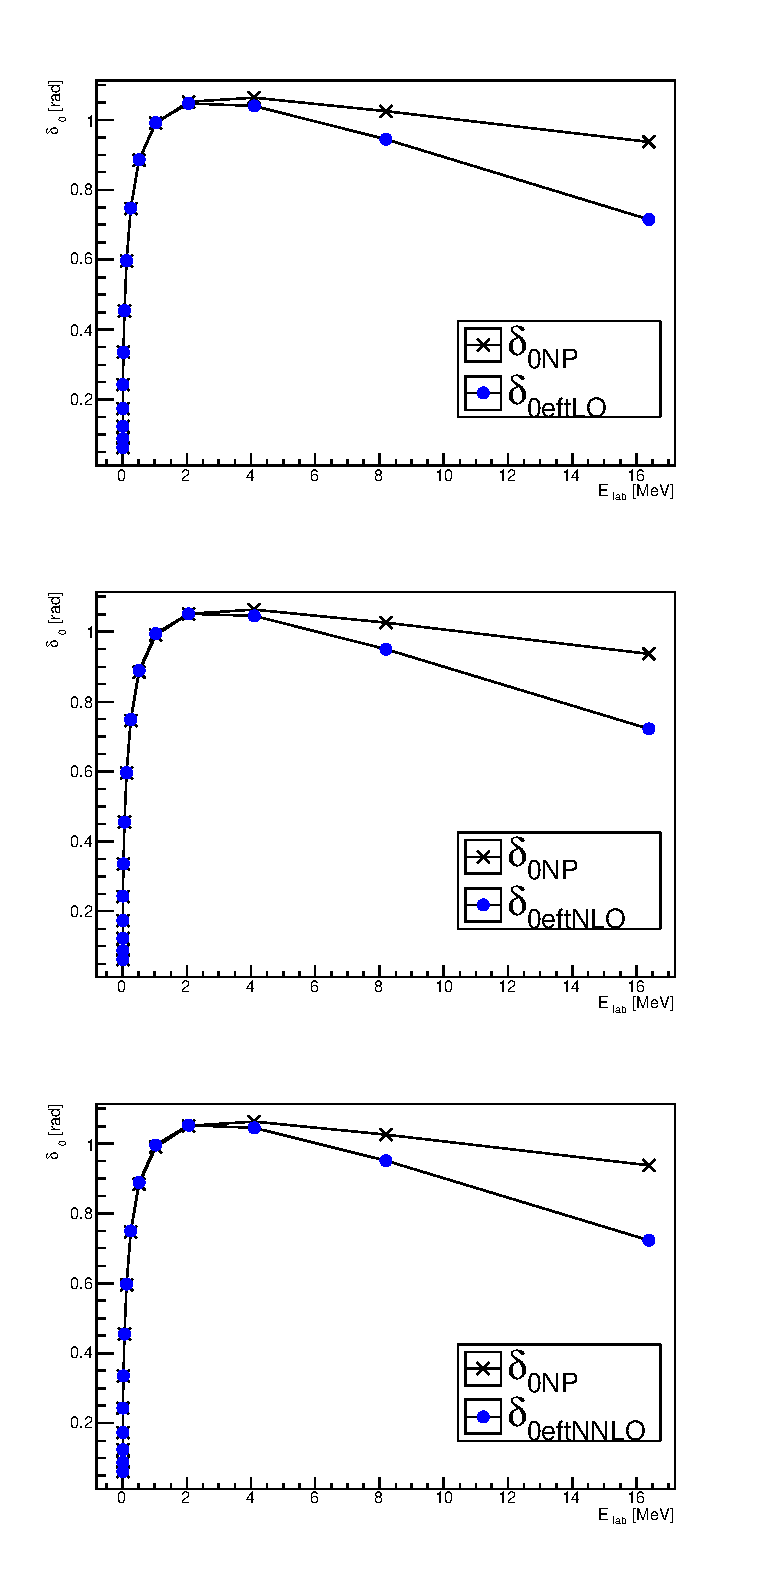
\includegraphics[width=0.5\textwidth]{figures/phy989_pionless.eps}
	\caption{Comparison between the three-Yukawa $np$ model $l=0$ phase shifts
	(black X)
	and the phase shifts calculated from the LO, NLO, NNLO EFT potentials (blue
	dots).}
	\label{fig:pionless}
\end{figure}

\begin{figure}
\centering
	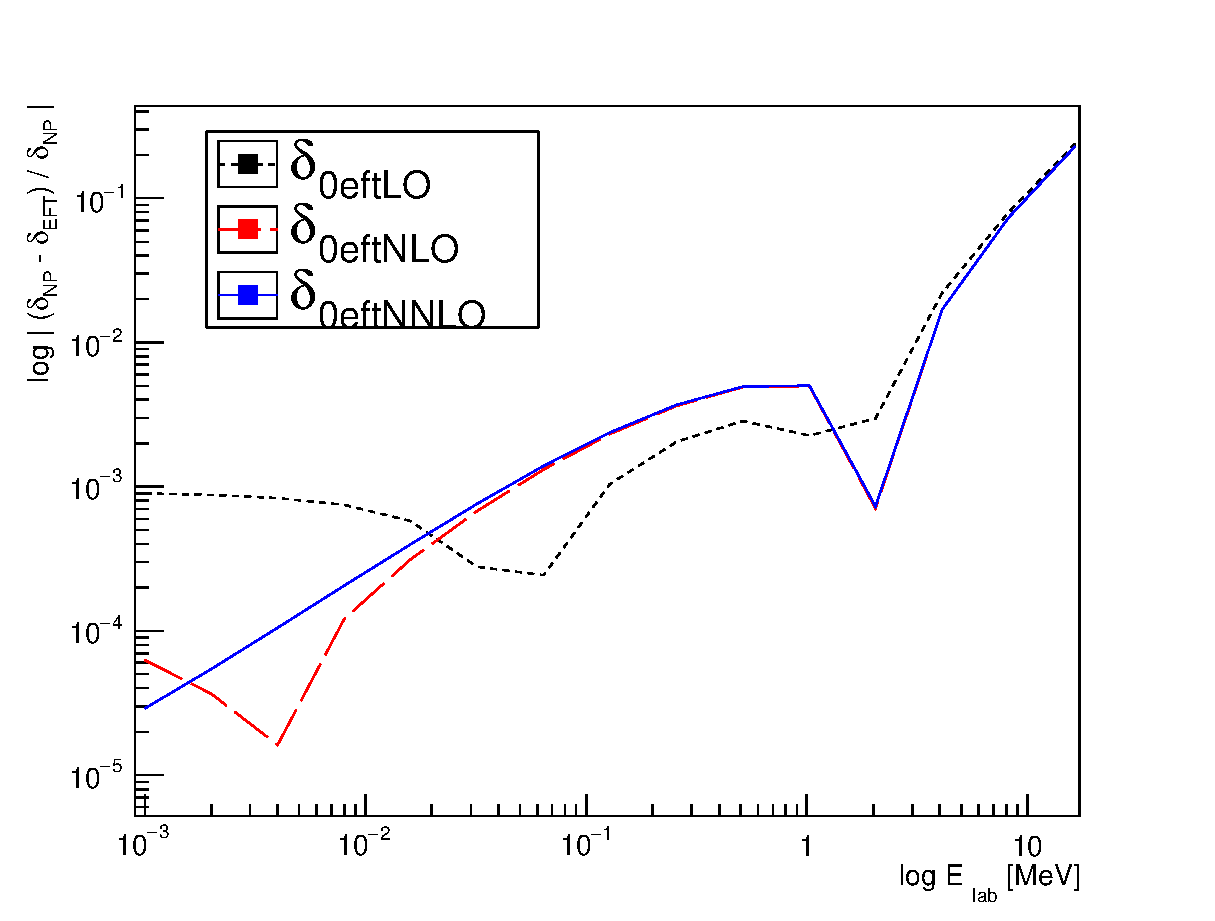
\includegraphics[width=0.5\textwidth]{figures/phy989_pionlessLepage.eps}
	\caption{Lepage error plot comparing the LO, NLO, NNLO EFT potentials to the
	$np$ model pseudo data. The kinks in the lines are where the sign of the error
	changes. The NLO and NNLO errors are the same above lab energies of 100
	keV.}
	\label{fig:pionlessLepage}
\end{figure}

\begin{table}
\centering
	\begin{tabular}{ c | c c }
	$\Lambda_c$ & $C_0$ & $C_2$\\
\hline
	0.07 & -2.5 & 180\\
	0.35 & -0.9 & -0.67\\
	0.71 & -0.86 & 3.6\\
	1.4 & -0.3 & 0.017\\
	2.1 & -0.196 & 4e-4\\
	7.1 & -0.01 & 0.01
	\end{tabular}
	\caption{Pionless EFT parameters for various values of the cutoff $\Lambda_c$.
	We note that the values for $C_0$ and $C_2$ are very cutoff dependent.}
	\label{tab:pionlessC0C2}
\end{table}

\begin{figure}
\centering
	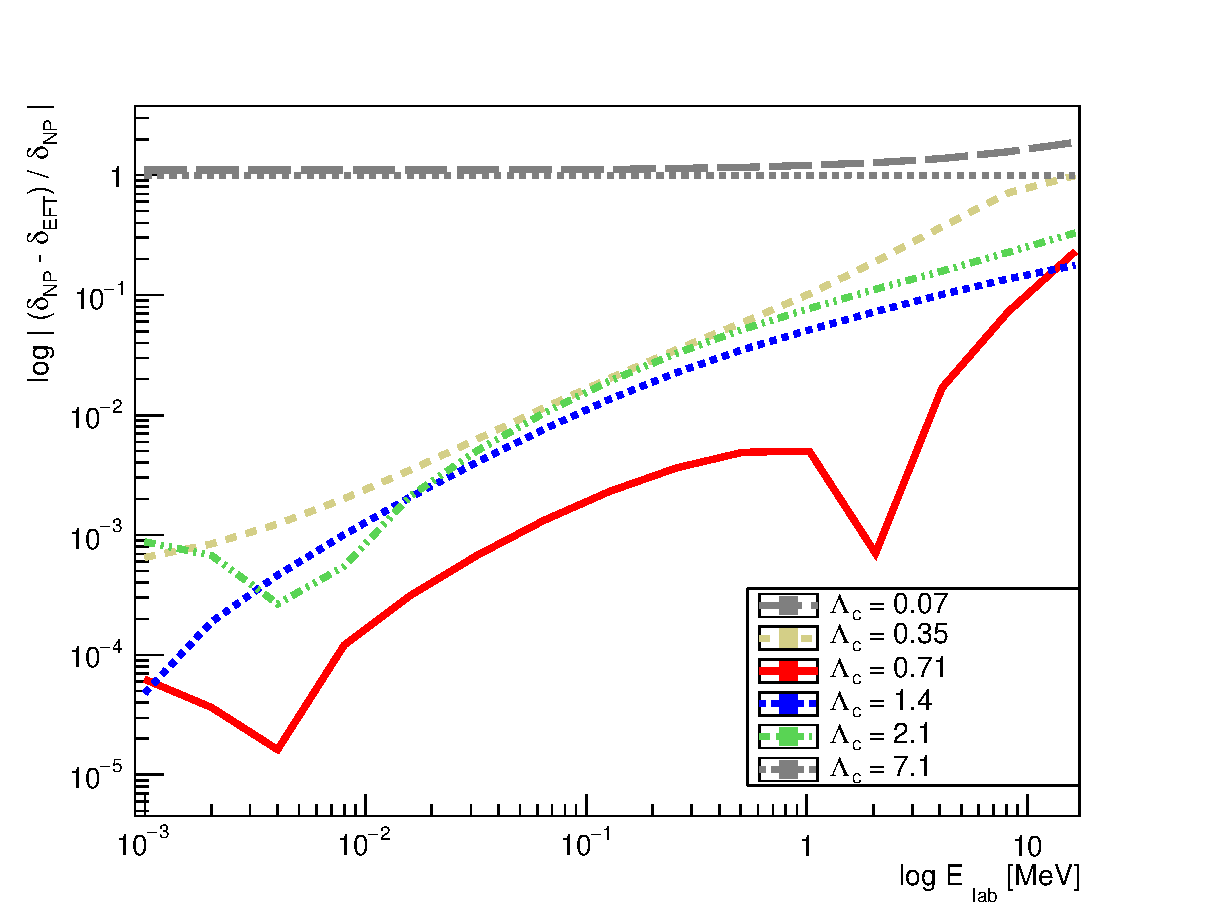
\includegraphics[width=0.5\textwidth]{figures/phy989_pionlessCutoff.eps}
	\caption{Lepage error plot for NLO EFT potentials with various cutoffs $\Lambda_c$.
	From these results, we deduce that $\Lambda_c = 0.71$ (the pion mass) is roughly
	the breakdown scale for which setting $\Lambda_c$ too far below or above this
	value worsens the agreement with the underlying theory.}
	\label{fig:LepageCutoff}
\end{figure}
	





\subsection{Including One-Pion Exchange}

We compare our phase shifts calculated with our one pion EFT to the $np$ model
in FIG.~\ref{fig:OnePion}. Note the better agreement with the pseudo data compared
to the pionless case in FIG.~\ref{fig:pionless}. Here we have set $\Lambda_c = 2.8$
fm$^{-1}$ since this is the range of second Yukawa term representing the high energy
physics that we're excluding from our EFT. We show a new Lepage error plot in
FIG.~\ref{fig:OnePionLepage}. Where we see features similar to those described
in the previous section. However, for the one-pion EFT, we see a more noticable
improvement from LO to NLO and from NLO to NNLO. Finally, we examine the effect
of changing $\Lambda_c$ in FIG.~\ref{fig:OnePionCutoff}; TABLE~\ref{tab:pionC0C2}
lists the coupling constants we used for each value of $\Lambda_c$. We see a
similar trend in the errors for different values of the cutoff although the one pion
EFT appears to be more stable in that doubling $\Lambda_c$ still produces as good
an agreement.




%%%%%%%%%%%%%%%
%%%%% PIONS !!! %%%%%
%%%%%%%%%%%%%%%

\begin{figure}
\centering
	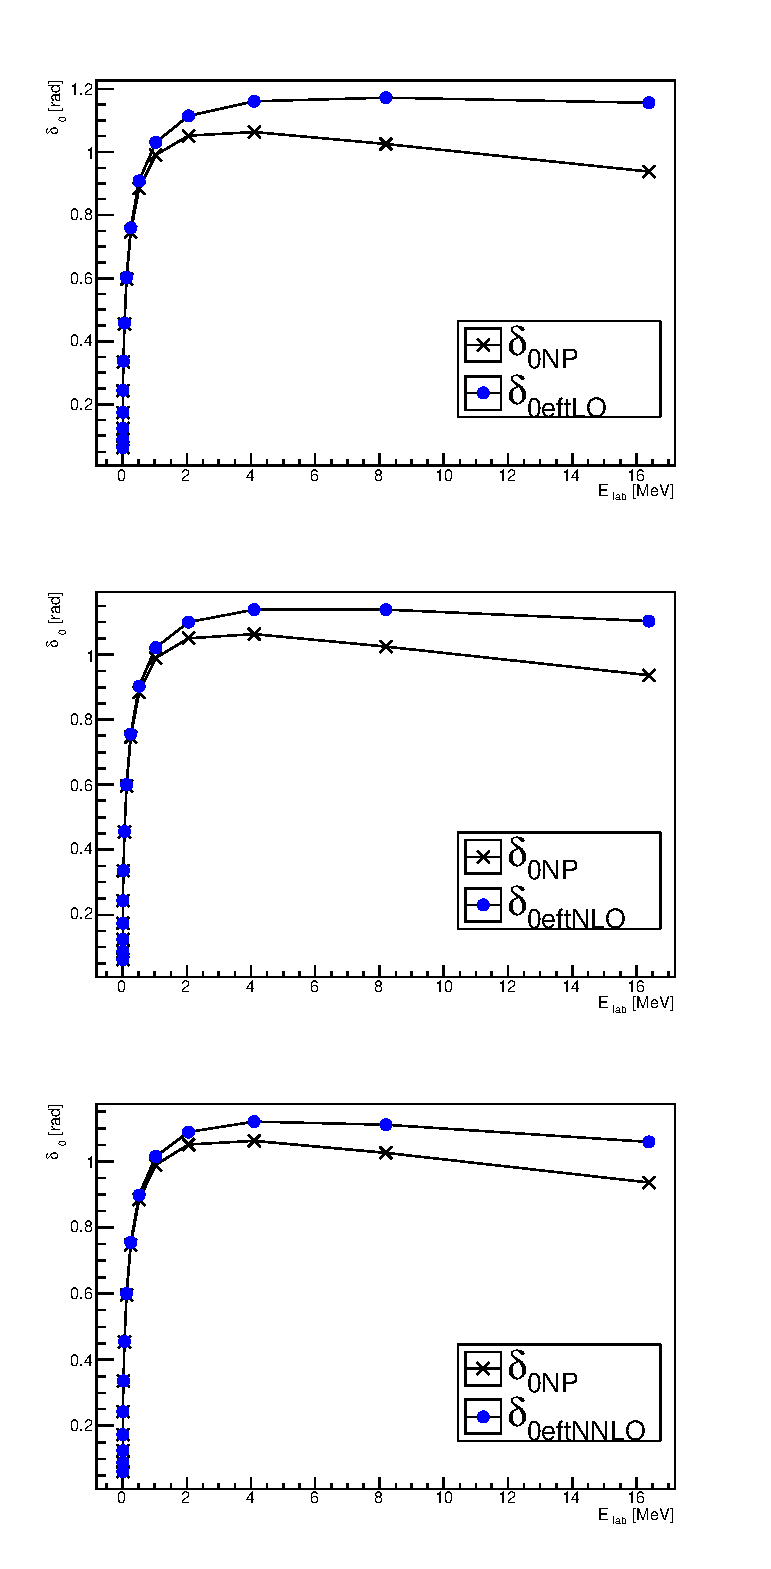
\includegraphics[width=0.5\textwidth]{figures/phy989_OnePion.eps}
	\caption{Comparison between the three-Yukawa $np$ model $l=0$ phase shifts
	(black X)
	and the phase shifts calculated from the LO, NLO, NNLO one-pion exchange
	EFT potentials (blue dots).}
	\label{fig:OnePion}
\end{figure}

\begin{figure}
\centering
	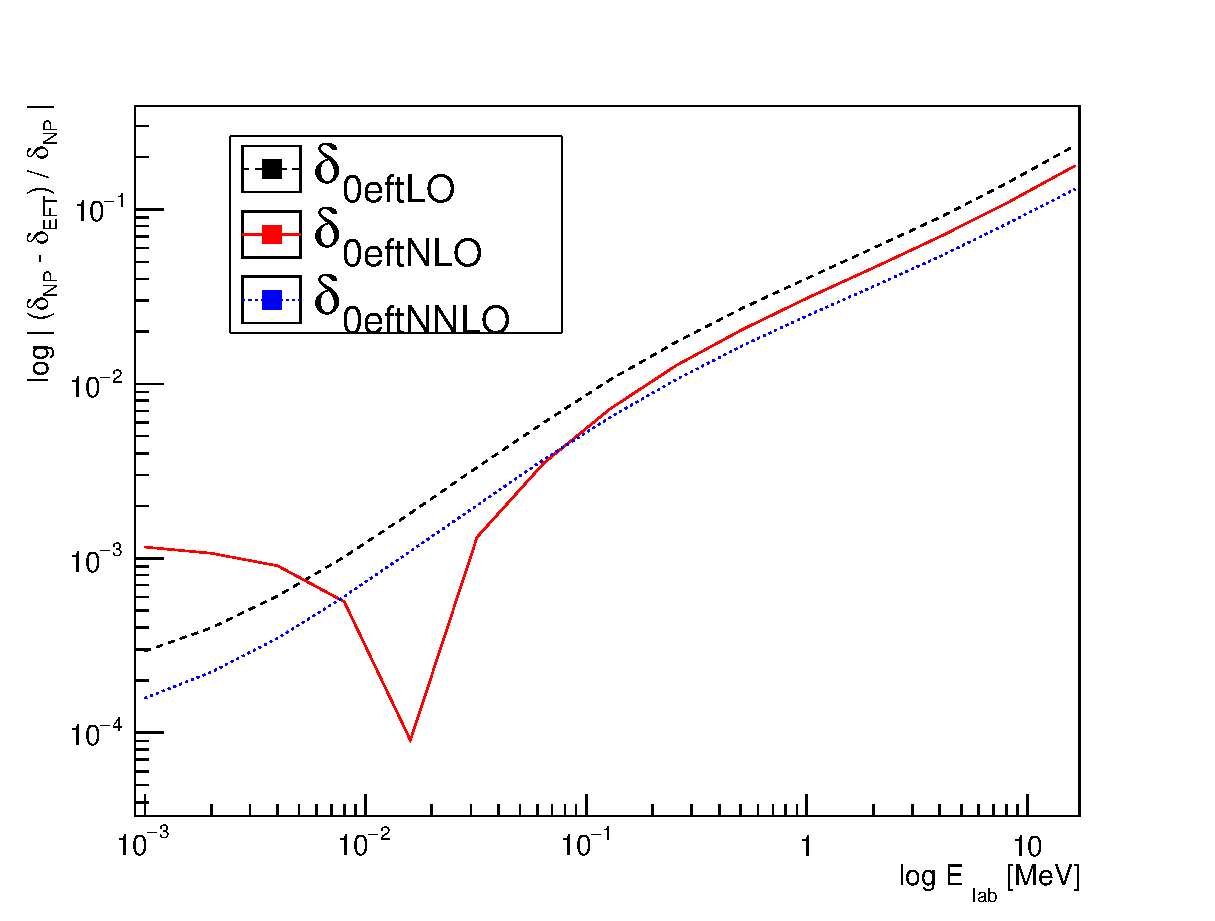
\includegraphics[width=0.5\textwidth]{figures/phy989_OnePionLepage.eps}
	\caption{}
	\label{fig:OnePionLepage}
\end{figure}

\begin{table}
\centering
	\begin{tabular}{ c | c c }
	$\Lambda_c$ & $C_0$ & $C_2$\\
\hline
	1.4 & -0.14 & 0.1\\
	2.8 & -0.13 & 0.93\\
	5.6 & 0.075 & 0.02\\
	10. & -0.048 & 0.002
	\end{tabular}
	\caption{One-pion EFT parameters for various values of the cutoff $\Lambda_c$.
	We note that the values for $C_0$ and $C_2$ are very cutoff dependent.}
	\label{tab:pionC0C2}
\end{table}


\begin{figure}
\centering
	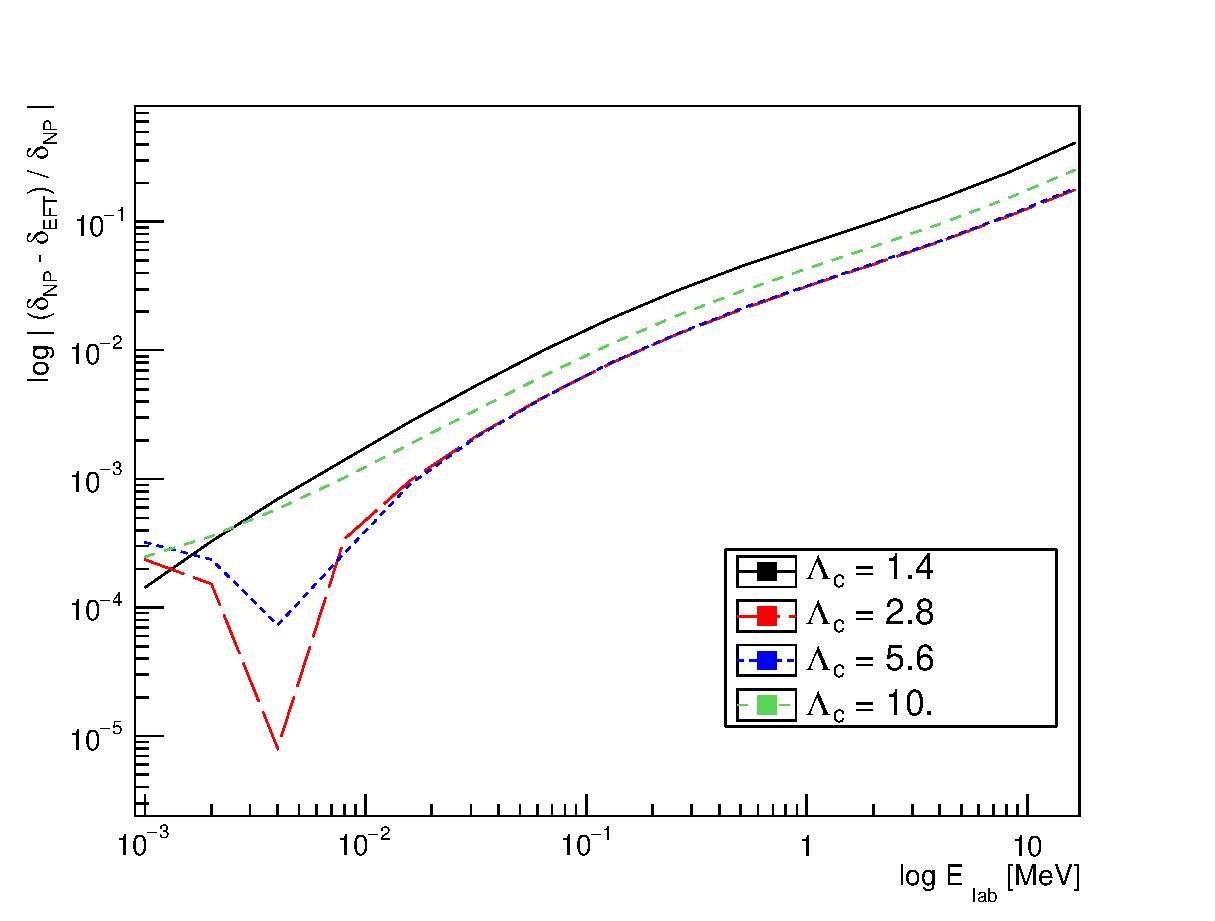
\includegraphics[width=0.5\textwidth]{figures/phy989_OnePionCutoff.eps}
	\caption{Lepage error plot comparing the $np$ model and EFT $\pi-$NLO with
	for various cutoff values $\Lambda_c$.}
	\label{fig:OnePionCutoff}
\end{figure}


\section{Conclusions}

We have crafted two versions of an effective field theory that approximates the physics of
neutron-proton scattering as it's described by the three-Yukawa potential model of the
previous project. By fitting to the low energy phase shifts of our underlying theory, we
extracted coupling constants for a pionless and one pion exchange version of an EFT. We
note that these were not rigorous fits and expect that improving them would improve
the agreement of our EFT with the phase shifts calculated using the underlying theory. In
each case we varied the cutoff momenta to find the energy scale at which the EFT breaks
down.

%\begin{thebibliography}{99}
%\bibitem{miller2006} G.~A.~Miller, A.~K.~Opper, and E.~J.~Stephenson, Annu.~Rev.~Nucl.~Sci.~{\bf 56}, 253 (2006).
%\bibitem{Morten} M. Hjorth-Jensen, Computational Physics Lecture Notes Fall 2015, August 2015.
%\bibitem{Mslides} M. Hjorth-Jensen, Computational Physics Notes, compphysics.github.io
%\bibitem{Golub1996} G. Golub, C. Van Loan, \textit{Matrix Computations} (John Hopkins University Press, 1996)
%\end{thebibliography}

\bibliographystyle{plainnat}
\bibliography{refs}

\end{document}
